\documentclass{article}
\usepackage[utf8]{inputenc}
\usepackage[russian]{babel}
\usepackage{graphicx}
\usepackage{wrapfig}
\usepackage{float}

\graphicspath{ {./data/images} }
\author{Александр Романов Б01-107}
\date{}
\title{3.4.1 Диа- и парамагнетики}

\begin{document}
\maketitle

\section{Введение}

    \subsection{Цель работы}
    Измерение магнитной восприимчивости диа- и парамагнитного образцов.

    \subsection{В работе используется}
    Электромагнит, весы, милливеберметр, регулируемый источник постоянного тока, образцы.

\section{Работа}
    \subsection {Подготовка}
    Для начала снимем зависимость магнитного потока Ф, пронизывающего милливеберметр от тока I:

    \begin{table}[H]
        \centering
    \begin{tabular}{|c|c|}
        \hline
        I, amp & B, mT \\\hline
        0,3  & 99     \\\hline
        0,6  & 185,3  \\\hline
        0,91 & 288,6  \\\hline
        1,20 & 372,5  \\\hline
        1,5  & 463    \\\hline
        1,81 & 545    \\\hline
        2,2  & 653,7  \\\hline
        2,6  & 735,2  \\\hline
        3,02 & 806,9  \\\hline
    \end{tabular}
    \end{table}

    \begin{figure}[H]
        \centering
        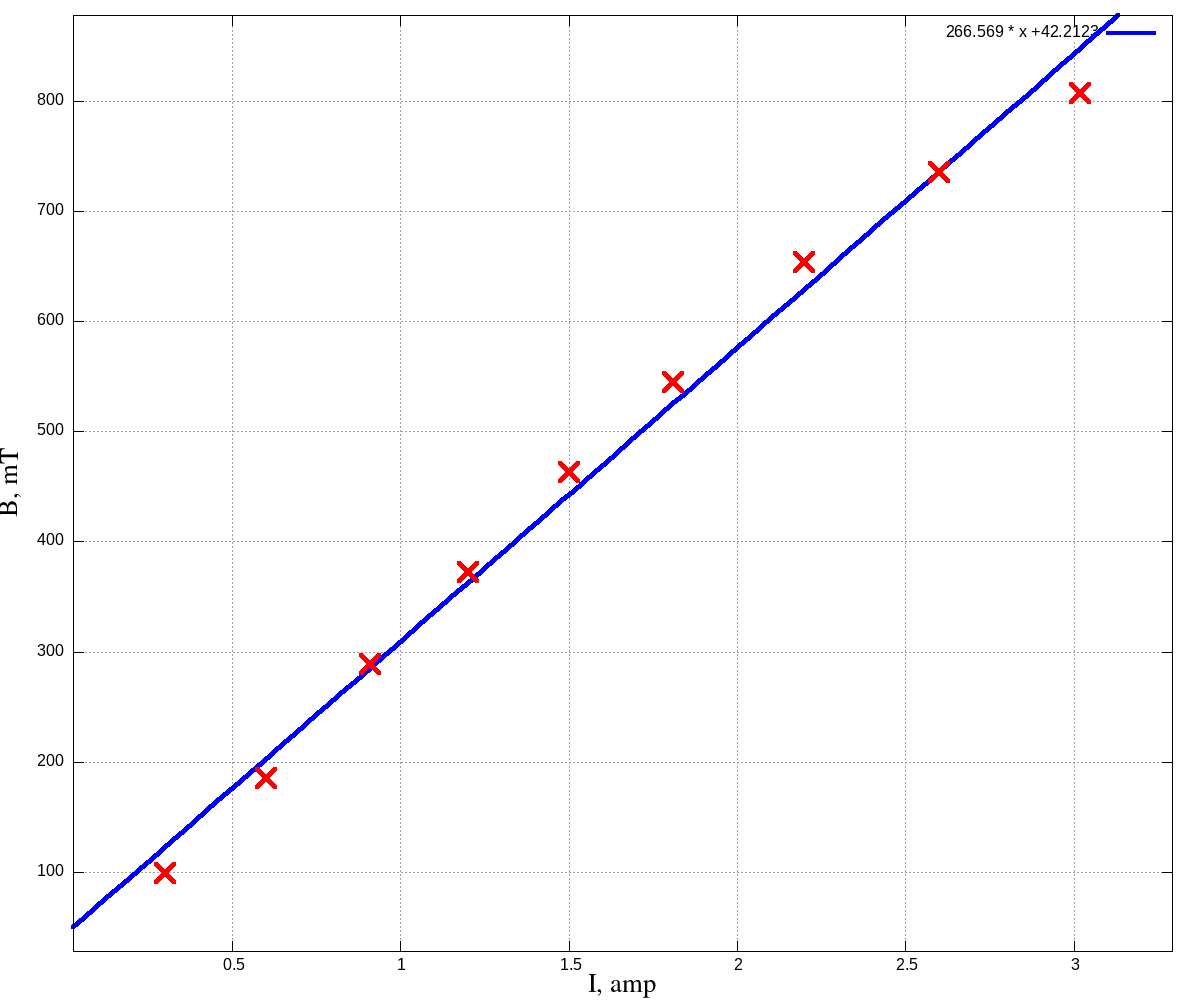
\includegraphics[width=\textwidth]{BI-comp.png}
        \caption{График B(I)}
    \end{figure}

    Результаты апроксимации уравнением вида \(y = kx + b\):
    \[ k = (266.7 \pm 42.2) \frac{mT}{amp} \]
    \[ b = (8.2 \pm 7.1) mT \]


    Запишем параметры образцов:

    \begin {table}[H]
        \centering
    \begin{tabular}{|c|c|c|}
        \hline
                & d, cm & m, g  \\\hline
        \(Al\)  & 1,00  & 25,2  \\\hline
        \(Cu\)  & 1,00  & 83,3  \\\hline
        \(Gr\)  & 1,00  & 11,   \\\hline
        
        
    \end{tabular}
    \end{table}


    Убедившись, что весы арретированы приступим к работе.

    \subsection{Измерения.}
    Будем измерять силу, действующую на образец в магнитном поле. Подвесим образец к весам,
    включим электромагнит и будем записывать показания. Результаты занесем в таблицу:

    \begin{table}[H]
    \centering
    \begin{tabular}{|c|c|c|c|}
        \hline
        & Cu         & Al       & Gr                   \\\hline
    $B^2$, $T^2$& \multicolumn{3}{|c|}{$\Delta$m, mg}    \\\hline
        0.010   & -1         & 0        & 7       \\\hline
        0.034   & -2         & 1        & 17      \\\hline
        0.083   & -4         & 4        & 25      \\\hline
        0.139   & -6         & 9        & 29      \\\hline
        0.214   & -8         & 14       & 30      \\\hline
        0.297   & -11        & 19       & 27      \\\hline
        0.427   & -15        & 28       & 16      \\\hline
        0.541   & -19        & 36       & 0       \\\hline
        0.651   & -24        & 46       & -21     \\\hline
    \end{tabular} 
    \end{table}

    Получим значение силы, действующей со стороны магнитного поля на образцы в ходе эксперимента:

    \begin{table}[H]
        \centering
        \begin{tabular}{|c|c|c|c|}
            \hline
            & Cu         & Al       & Gr                       \\\hline
        $B^2$, $T^2$& \multicolumn{3}{|c|}{F, uN}              \\\hline
            0.010   & -9.8          & 0           & 68.6       \\\hline
            0.034   & -19.6         & 9.8         & 166.6      \\\hline
            0.083   & -39.2         & 429.2       & 245        \\\hline
            0.139   & -58.8         & 88.2        & 284.2      \\\hline
            0.214   & -78.4         & 137.2       & 294        \\\hline
            0.297   & -107.8        & 186.2       & 264.6      \\\hline
            0.427   & -147          & 274.4       & 156.8      \\\hline
            0.541   & -186.2        & 352.8       & 0          \\\hline
            0.651   & -235.2        & 250.8       & -205.8     \\\hline
        \end{tabular} 
        \end{table}

    \subsection{Обработка экспериментальных данных.}

    Построим графики зависимости $|F|(B^2)$:

    \begin{figure}[H]
        \centering
        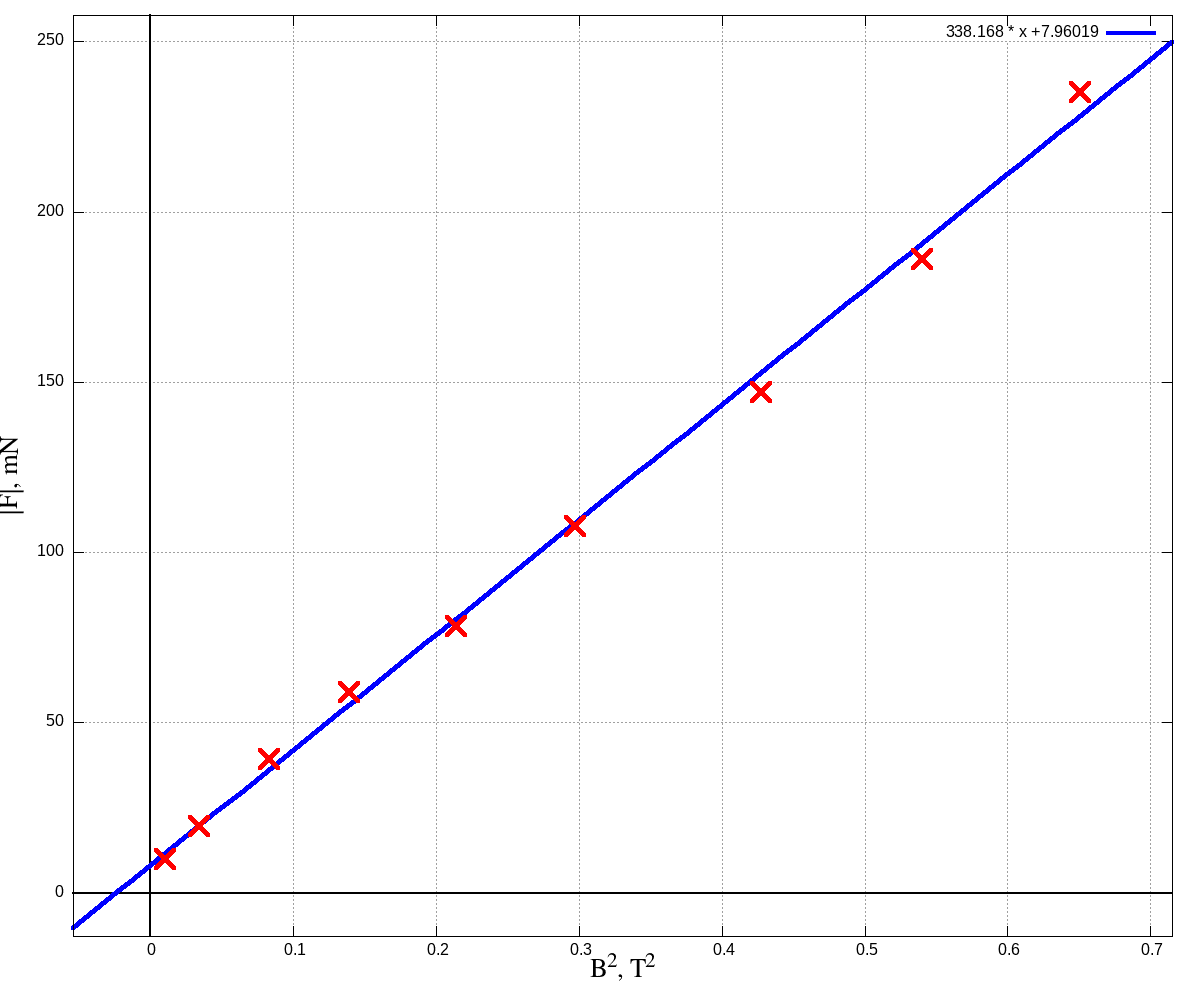
\includegraphics[width=\textwidth]{Cu-comp.png}
        \caption{$|F|(B^2)$ для Cu}
    \end{figure}

    Результаты апроксимации уравнением вида \(y = kx + b\):
    \[ k = (338.2 \pm 10.9) \frac{uN}{T^2} \]
    \[ b = (-13.3 \pm 2.36) uN \]

    Из формулы
    \[ F \simeq \chi\frac{B_0^2}{2\mu_0}S \]

    Вычислим значение удельной магнитной восприимчивости \(\chi^m\) для Меди:
    \[ \chi^m = \frac{2\mu_0F}{B_0^2S\rho} \]

    Взяв значение \( \mu_0 = 4\pi \cdot 10^{-7} H/m \), \( \rho_{Cu} = 8940 kg/m^3 \) и учтя, что медный стержень
    выталкивался из магнита получим:
    \[ \chi^{m}_{Cu} = (-1.2 \pm 0.04) \cdot 10^{-9} m^3/kg \]

    Это значение отличается от табличного (\( \chi^m_{Cu} = -0.086 \cdot 10^{-9} m^3/kg \)) больше чем на погрешность
    измерения, однако всё ещё довольно близко. Это может быть связано с неидеальность образца или тем что не была учтена
    погрешность измерения весов.

    \begin{figure}[H]
        \centering
        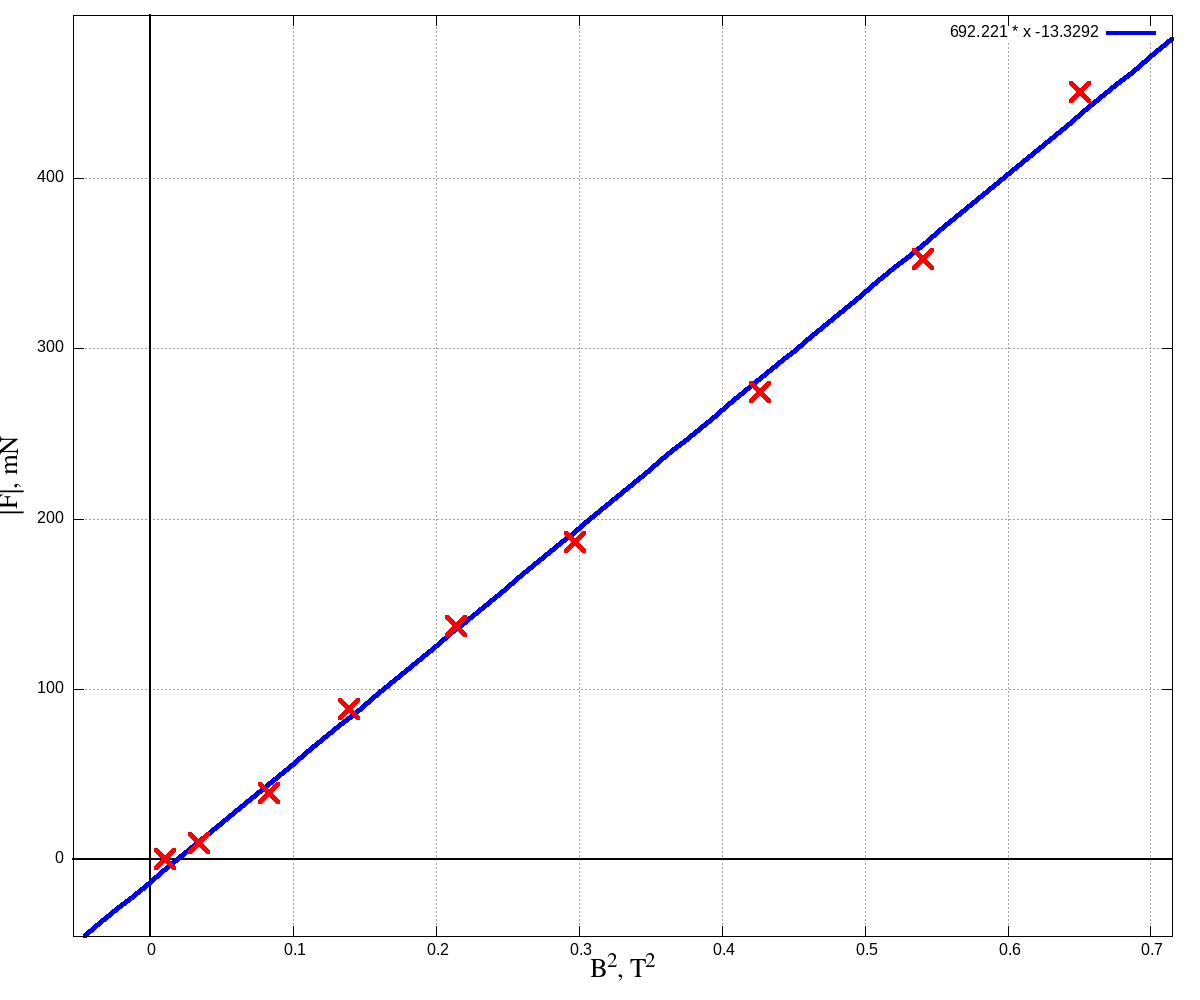
\includegraphics[width=\textwidth]{Al-comp.png}
        \caption{$|F|(B^2)$ для Al}
    \end{figure}

    Результаты апроксимации уравнением вида \(y = kx + b\):
    \[ k = (692.2 \pm 5.9) \frac{mN}{T^2} \]
    \[ b = (7.96 \pm 1.3) mN \]

    Из формулы
    \[ F \simeq \chi\frac{B_0^2}{2\mu_0}S \]

    Вычислим значение удельной магнитной восприимчивости \(\chi^m\) для алюминия:
    \[ \chi^m = \frac{2\mu_0F}{B_0^2S\rho} \]

    Взяв значение \( \mu_0 = 4\pi \cdot 10^{-7} H/m \); \( \rho_{Cu} = 2700 kg/m^3 \) и учтя, что алюминиевый стержень
    втягивался в магнит получим:

    Разделим на плотность (\( \rho_{Cu} = 2700 kg/m^3 \)) и получим удельное значение:
    \[ \chi^{m}_{Al} = (+8.2 \pm 0.07) \cdot 10^{-6} m^3/kg \]

    Это значение отличается от табличного (\( \chi_{Cu} = +0.61 \cdot 10^{-9}m^3/kg  \)) на 2 погрешности. Эту разницу можно объяснить
    неидеальностью образца и тем, что не была учтена погрешность измерения весов.

    
    \begin{figure}[H]
        \centering
        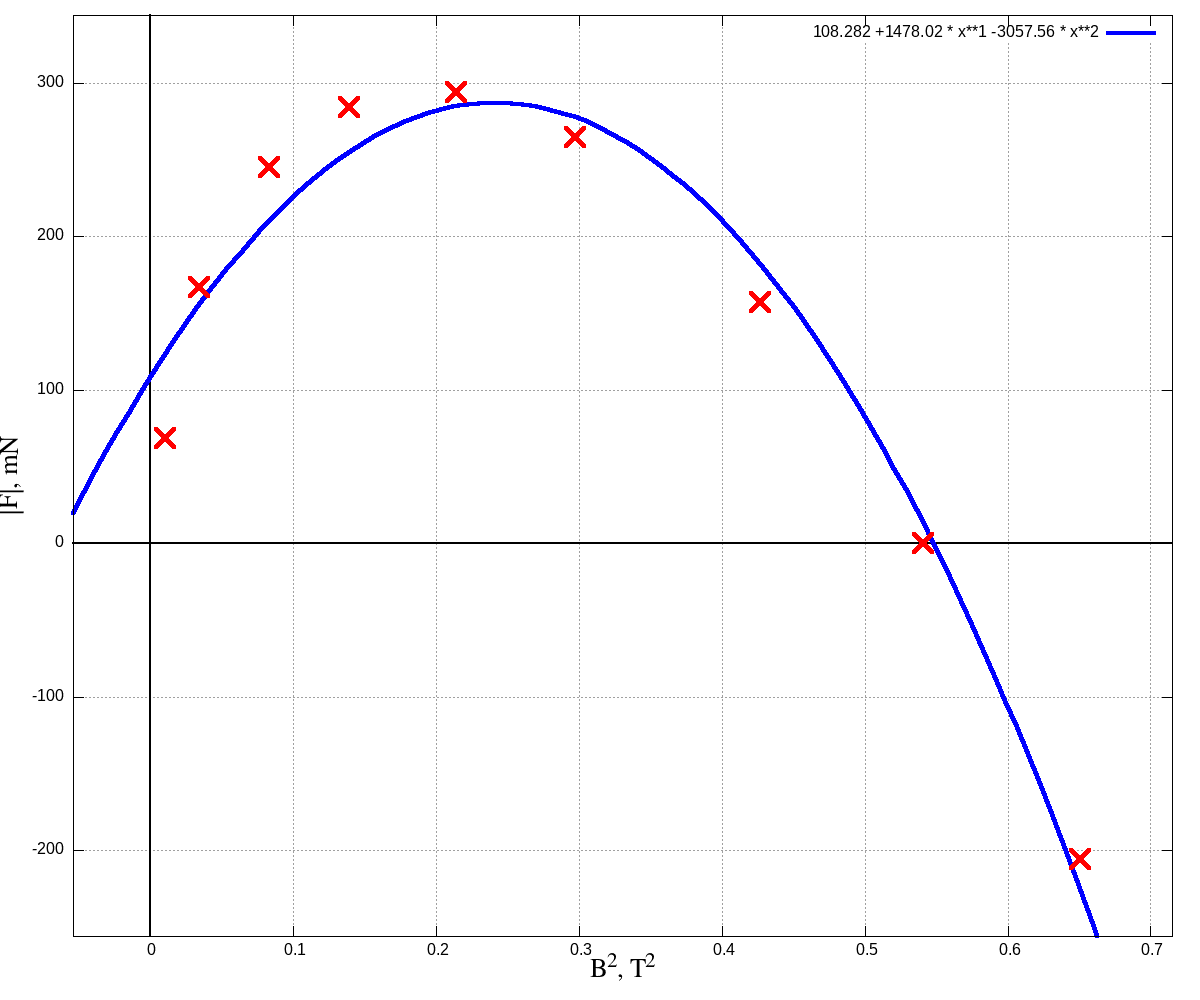
\includegraphics[width=\textwidth]{Gr-comp.png}
        \caption{$|F|(B^2)$ для Gr}
    \end{figure}

    Результаты апроксимации уравнением вида \(y = ax^2 + bx + c\):
    \[ a = (-3057.56) \frac{uN}{T^4} \]
    \[ b = (1478.02) \frac{uN}{T^2} \]
    \[ c = (108.282) uN \]

    Поведедние же графита не поддаётся той же линейной апроксимаии и в неплохо описывается многочленом второй степени.

    \section {Выводы}
    \begin{enumerate}
        \item Были вычислены значения удельной магнитной восприимчивости для меди и алюминия. Полученные
    значения отличаются от табличных больше чем хотелось бы. Это монжо объяснить тем, что не была учтена погрешность
    даваемая весами. Однако данные всё ещё довольно точны и по ним можно сказать (по знаку $\chi^m$), что медь
    относится к классу диамагнетиков, а алюминий - к классу парамагнетиков.
        \item Было также обнаружено, что Графит ведёт себя координально другим образом относительно меди
    и алюминия. Сила действующая на него зависит квадратично от \(B^2\). Что может свидетельствовать о том,
    что графит является не совсем обычным диа- или парамагнетиком. Возможно он обладает некоторыми феромагнитными
    свойствами.

    \end{enumerate}



\end{document}